\chapter{Introduction to Electromagnetic Waves}
\begin{figure}[h]
\centering
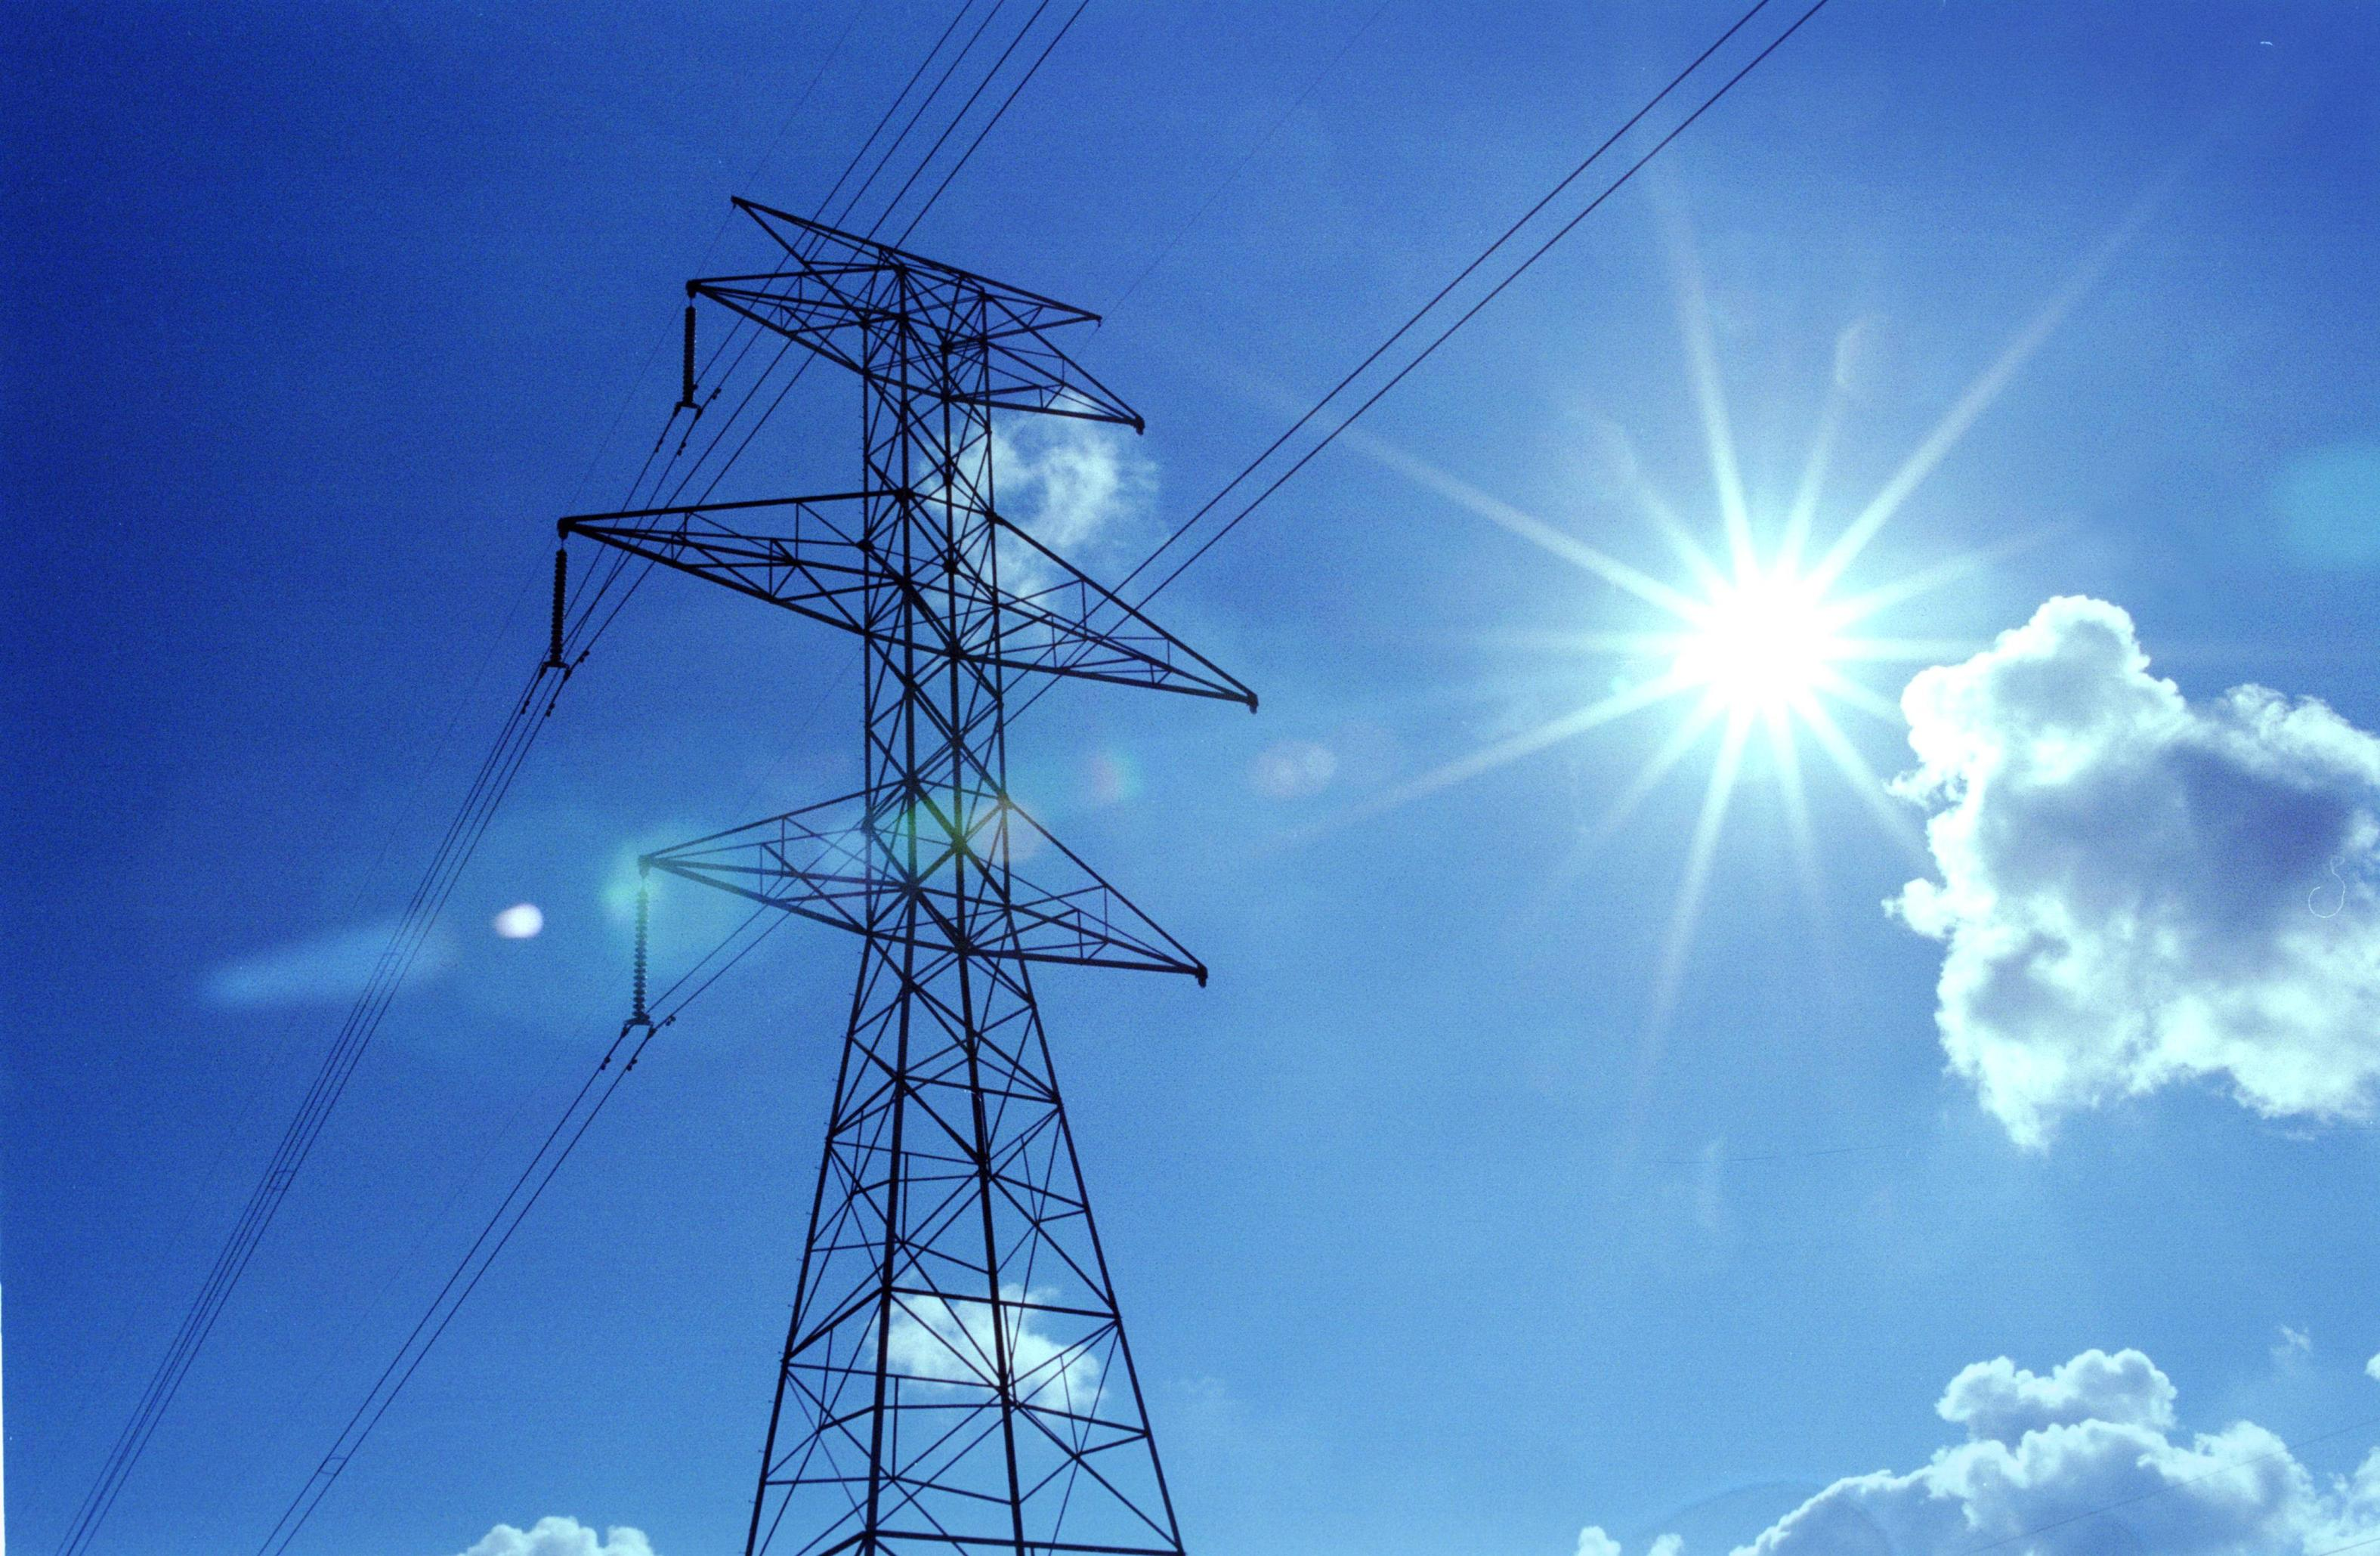
\includegraphics[width=1\linewidth]{./graphics/transmission1}
\caption{Overhead transmission line}
\end{figure}


The concept of electromagnetic waves has fascinated man for so many years that man has asked so many questions varying from "Why do stars twinkle?", to "Why do magnetic needles deflect?", and "Why does light travel from the sun when there is no medium between?"\newline

In modern-day, questions vary from "how do we have tv reception?" to "how do we have radio stations operating" to "how does a mobile phone work?", "why are certain things halted when they are kept inside a microwave". All these phenomena revolve around the concept of electromagnetic waves.\footnote{The concept of electromagnetic waves is virtually applied in almost all advanced technology.}\\

Electromagnetic waves can be divided into;
\begin{enumerate}
\item low frequency and high power
\item high frequency and low power
\end{enumerate}


In this course, we shall concentrate on the high-frequency and low-power properties of electromagnetic waves. Devices and phenomena like electrical machines, electrical power generators, transformers, and distribution of electrical energy fall into the category of low-frequency high power. Whereas modern systems, like mobile communication, radars, satellite, and optical fibres, fall into the high-frequency low-power category. So we are mainly going to investigate what happens as frequency increases in electromagnetic waves\footnote{When the frequency of a wave increases, the wavelength will decrease to compensate for this increment} and how they can be transmitted from one position to another without loss.\\

Electromagnetic waves see applications in many areas namely\footnote{The application of electromagnetic waves are not limited to this list but for this course, we streamline the application to these few.}:
\begin{enumerate}
\itemsep0em
\item Transmission lines and HF circuits.
\item Antennas.
\item Satellite communication.
\item Fibre-optic communication.
\item Radars.
\item Radio astronomy.
\item Electromagnetic Interference/Compatibility(EMI/EMC)
\end{enumerate}

We intend to investigate the behavior of time-varying electrical and magnetic fields especially when the frequency of operation is large. This investigation is going to be based on maxwell's four equations of electromagnetic waves\footnote{see chapter 17 for detailed expression of maxwell's equations}. However, as we proceed certain approximations can be used to investigate the same phenomenon in terms of voltage and current which are electrical circuits.\\

\begin{figure}[h]
\centering
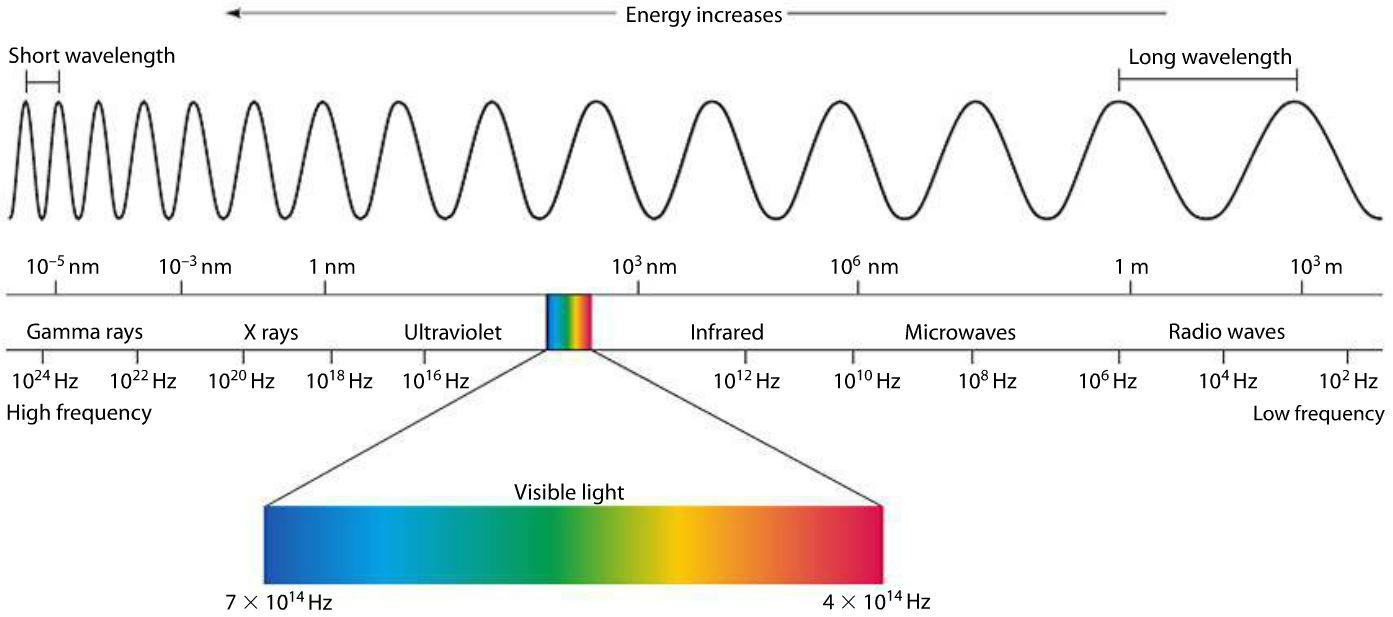
\includegraphics[width=1\linewidth]{./graphics/electromagneticspectrum}
\caption{The electromagnetic spectrum}
\label{fig:electromagneticspectrum}
\end{figure}

\textbf{Electromagnetic spectrum:} The word electromagnetic spectrum corresponds to any phenomenon which relates the time-varying signals and time-varying electric or magnetic fields \textit{electromagnetic spectrum shown in Figure~\ref{fig:electromagneticspectrum}}. Any wave no matter how small can be put in the category of time-varying electric or magnetic fields. The entire frequency range from very low frequencies to very high frequencies can be summarized as \textbf{radio frequencies}.\\

\section{Transmission lines and High-frequency circuits}

Depending on the frequency of operation, there are different media to transmit electromagnetic waves. When the frequency is between 30MHz to 300MHz, the coaxial cable is used for transmission of the wave, from 30GHz to 300GHz the structure used is called a waveguide and as the frequency goes high the media used is the optics fibre.

A question that comes to mind in electromagnetic wave transfer is "Why do we have to increase frequency?" If the major application of high frequency is in communication, then for transmitting more information we require large bandwidth. Since the frequency of operation is proportional to the bandwidth, by increasing the frequency of operation we increase the bandwidth and as such one can transmit more information on a given channel.
\begin{figure}[h]
\centering
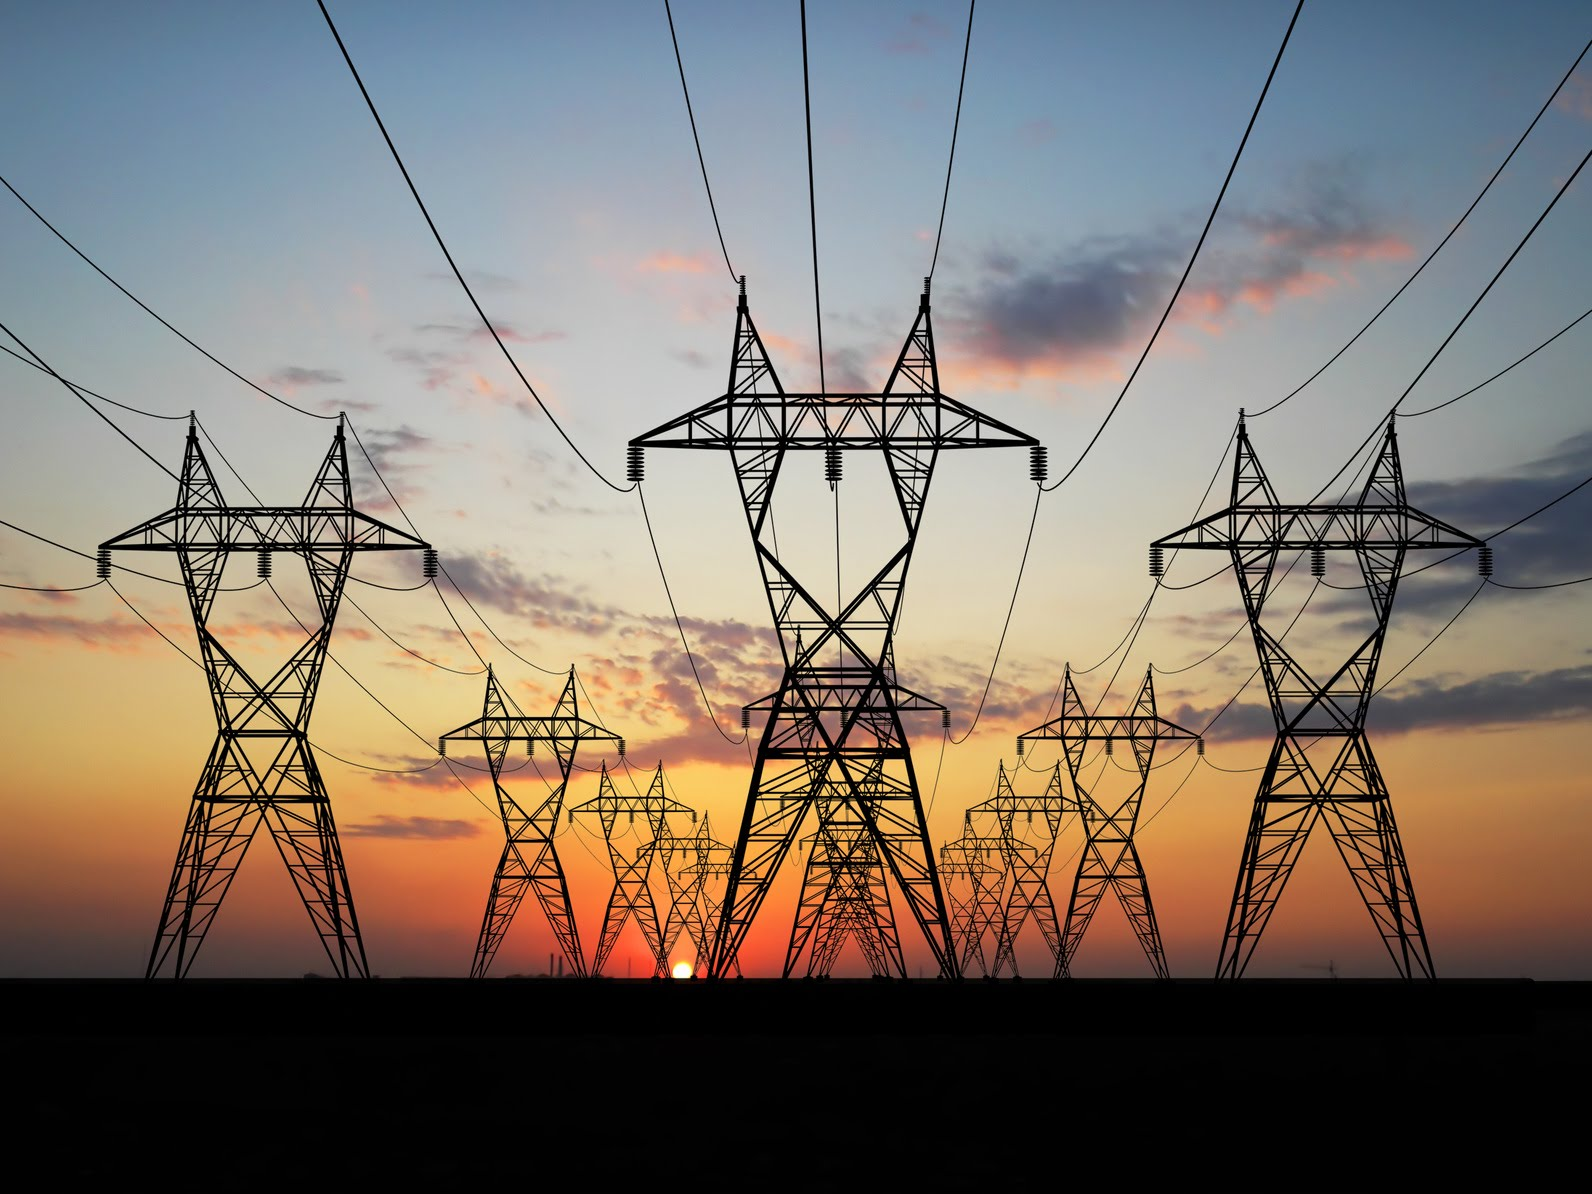
\includegraphics[scale=0.1]{./graphics/transmission2}
\caption{Power transmission line}
\end{figure}

\textbf{Transmission line:} In transmission lines, our main concern is how voltage and current would flow in a two-conductor system called a \textit{transmission line} and how losses occur during transmission \footnote{when the frequency of a wave increases its wavelength decreases and when the wavelength of the wire is comparable to the length of the transmitting media (length of the wire) the losses along the wire becomes too significant to ignore.}.

There are different types of transmission media and the application of this media is based on the frequency range of the signal. \begin{figure}[h]
\centering
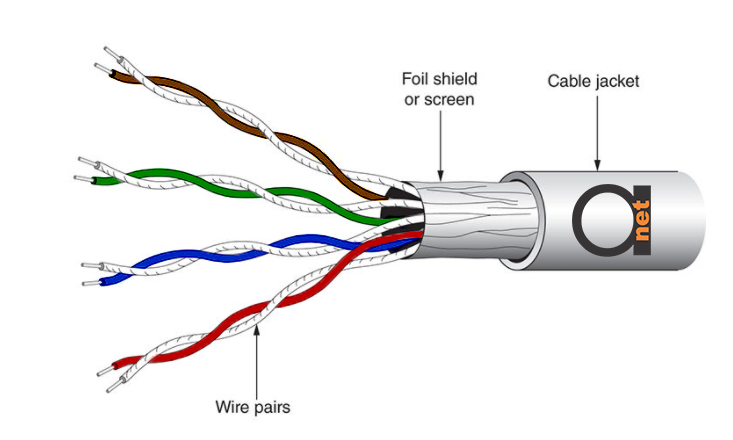
\includegraphics[width=1\linewidth]{./graphics/twistedpairs}
\caption{Twisted pair of wires}
\end{figure} 

\textbf{Twisted pairs:} They are point to point transmission lines\footnote{connections between two nodes or endpoints} (it is a balanced transmission line having voltages $v^{+}$ and $v^{-}$ connected at its terminals). An example of the twisted pairs is the telephone wires; it characterizes low data rate, high EMI and is lossy at Radio frequency.

\textbf{Coaxial cable:} For the coaxial cable we have an example in the LAN cable; it characterizes data rates of up to a few Mbps, low EMI and moderate loss.
\begin{figure}[h]
\centering
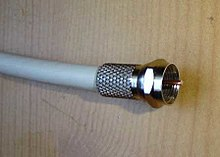
\includegraphics[scale=0.4]{./graphics/coaxialcable}
\caption{Coaxial cable}
\end{figure}

\textbf{Wave guides:} These are hollow circular or rectangular pipes and they are used when the frequency becomes high in other to reduce losses. 

Inside the hollow metal conductor, an electromagnetic wave can propagate and here rigorous analysis of electromagnetic wave propagation is carried out to help find out what the field distribution would look like and how much energy loss will take place inside.
\begin{figure}[h]
\centering
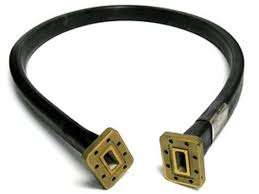
\includegraphics[scale=0.4]{./graphics/waveguide2}
\caption{Wave guide}
\end{figure}

\section{Antennas}
\begin{figure}[h]
\centering
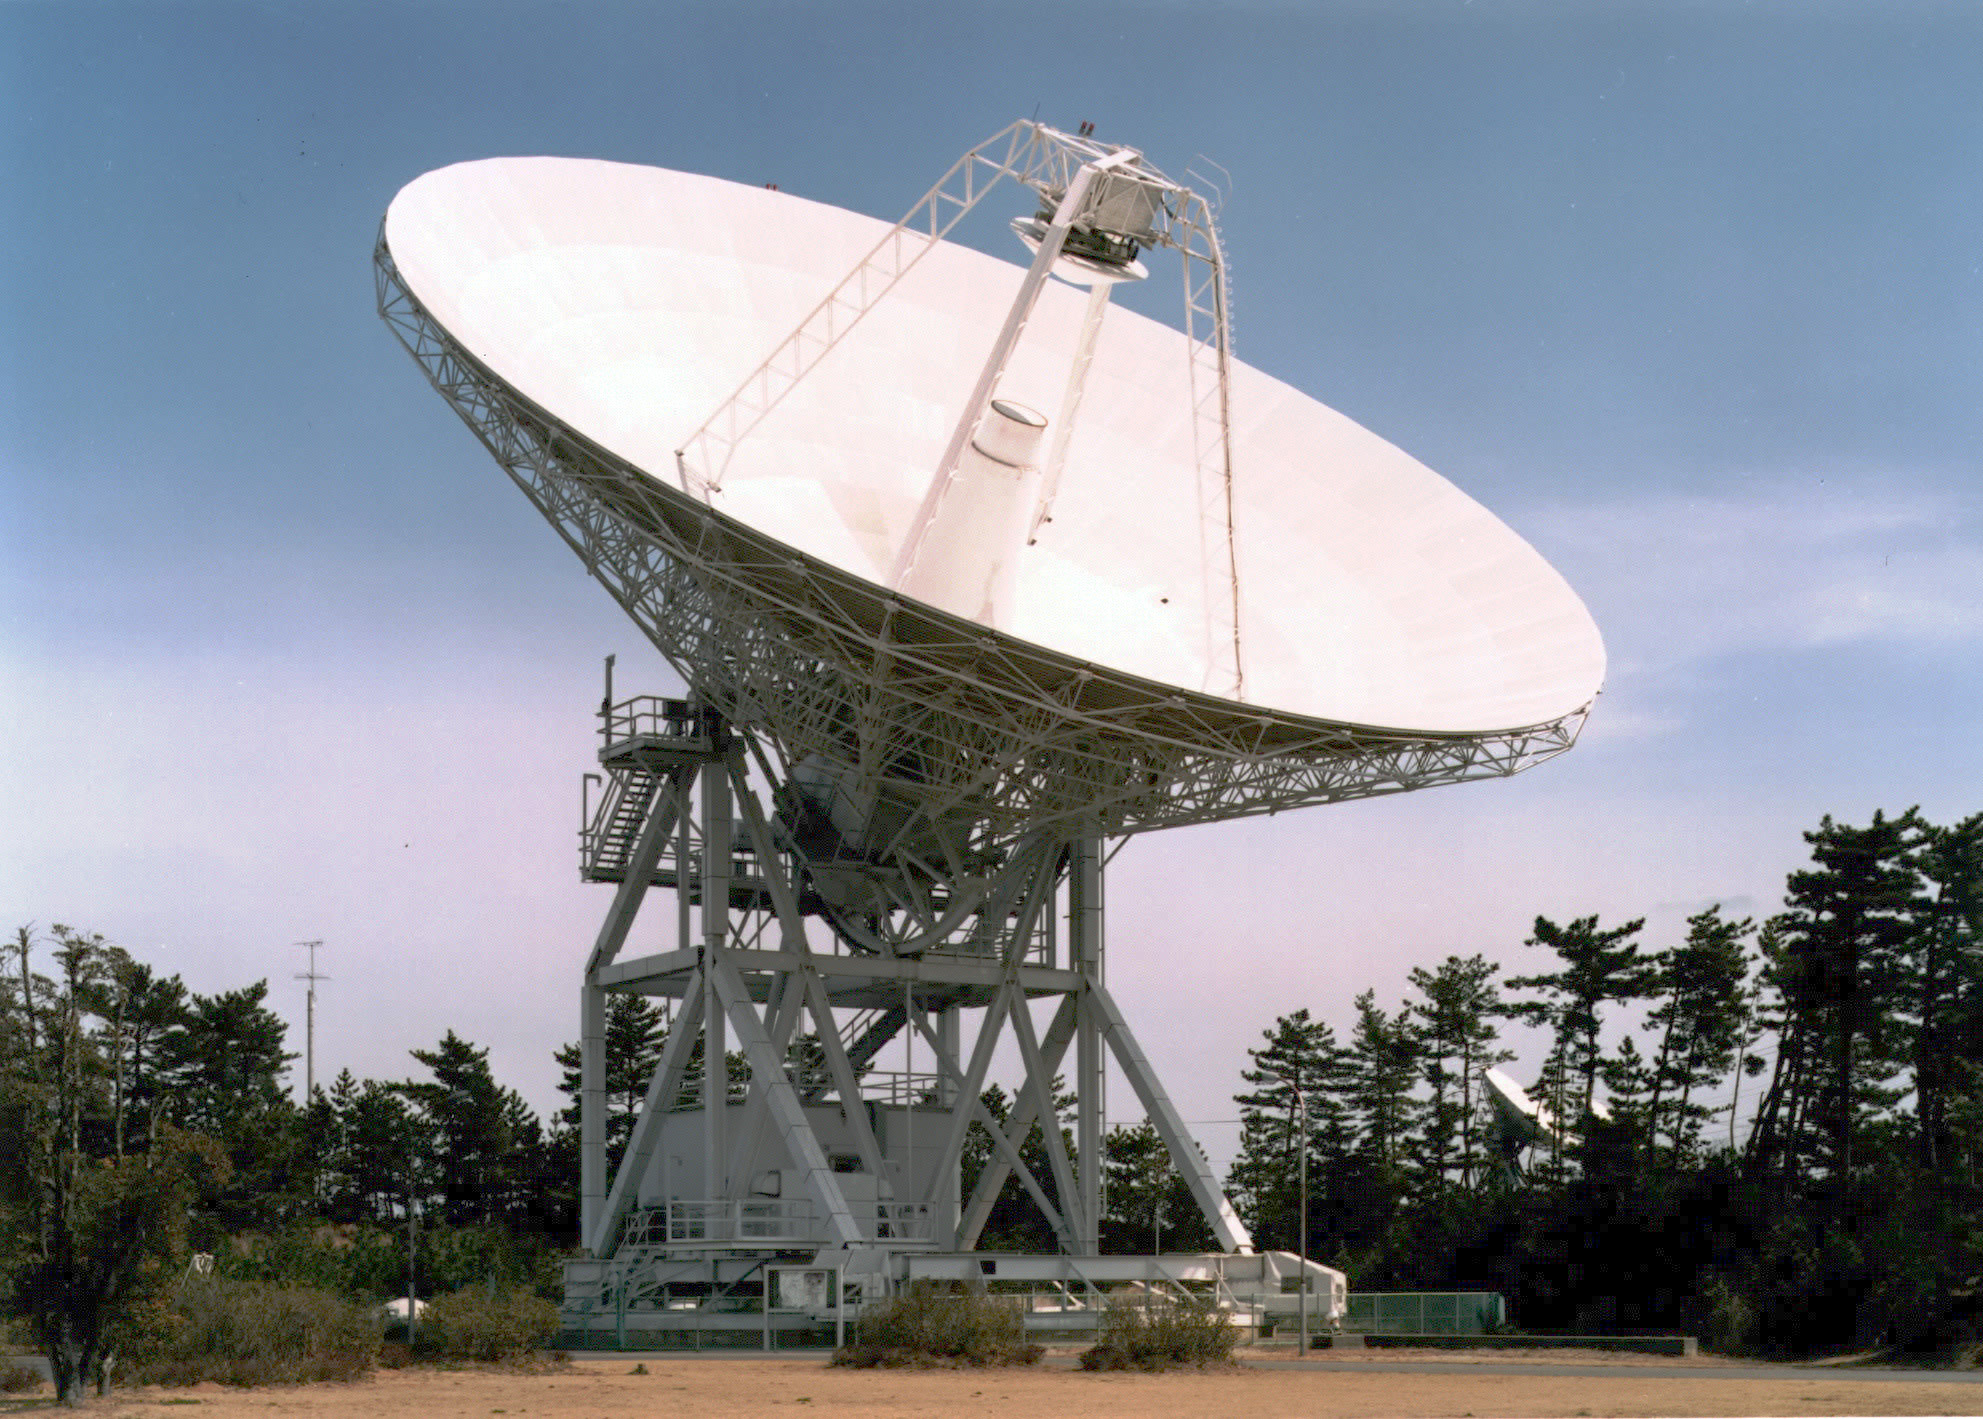
\includegraphics[scale=0.4]{./graphics/spcaceantenna}
\caption{Parabolic dish antenna}
\end{figure}
An antenna is a device which can transmit electromagnetic energy into space and also can receive electromagnetic energy coming from space. An example is the parabolic dish antenna, signals coming from a point are like parallel rays when it gets to the parabolic dish antenna the rays converge to a focal point called the feed from there they get processed into an electrical signal.\\

An antenna is a device which separately puts radiation in the desired direction. A simple antenna structure may not necessarily provide the desired characteristics of modern-day smart antenna systems where radiation characteristics can be automatically changed to maximize the reception of the signal.\\

Other more advanced antenna systems referred to as the \textbf{smart antennas} can selectively push the radiation in the desired direction. There are two types of smart antennas which are the \textbf{adaptive array} and \textbf{switched beam systems}.\\

\textit{\textbf{adaptive array}}
This antenna steers the beam in the direction of the user/transmitter while simultaneously nulling interfering signals.
\begin{figure}[h]
\centering
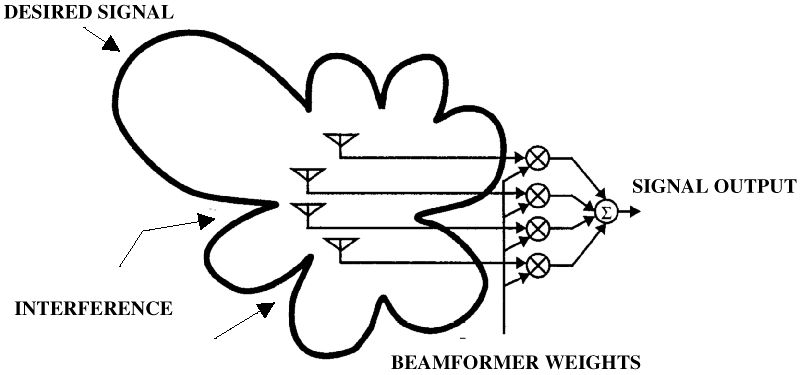
\includegraphics[scale=0.3]{./graphics/fh06_02}
\caption{Adaptive array system}
\end{figure}

\textit{\textbf{switched beam antenna}} has multiple beams which can be switched depending on the area an observer is situated. A signal can be transmitted or received from that zone. Therefore, depending on the requirement of the system a beam is selected hence the name switched beam.
\begin{figure}[h]
\centering
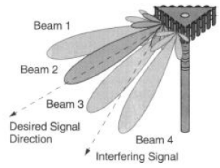
\includegraphics[scale=0.7]{./graphics/switchedbeam}
\caption{Illustration of a switched beam antenna}
\end{figure} 

\section{Satellite communication}
A satellite is an object that is placed above the earth's surface. The satellite station on the earth's surface is usually called the earth station which transmits signals from the earth to satellites and also receives signals from the satellite to the earth. Certain frequency bands are assigned for satellite communication. Satellite communication is a point-to-multi-point system.
\begin{figure}[h]
\centering
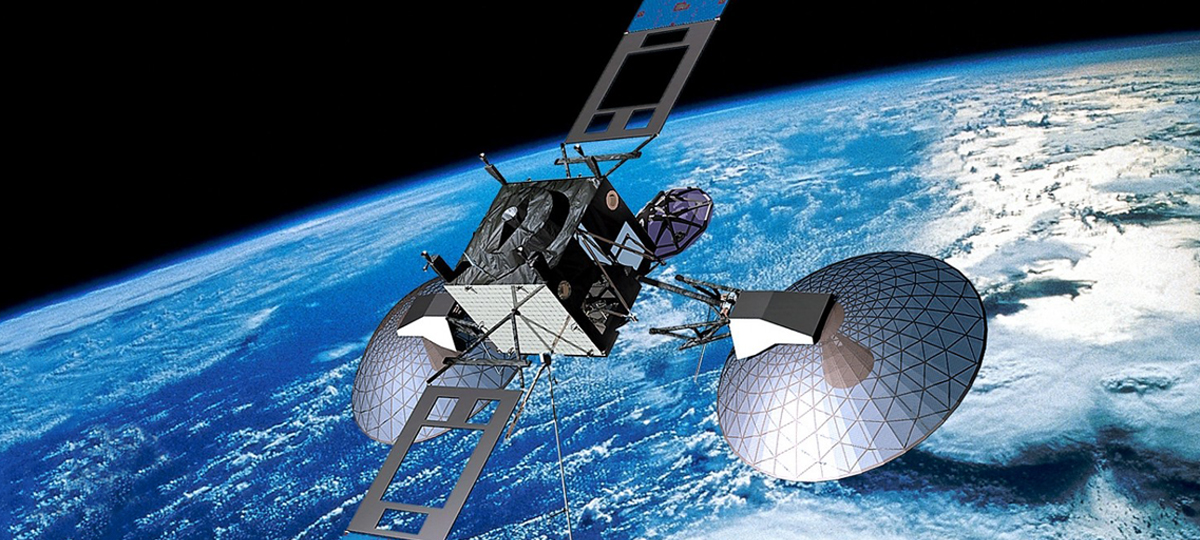
\includegraphics[scale=0.2]{./graphics/satellite}
\caption{Space satellite}
\end{figure}

The whole propagation of the electromagnetic wave and proper placing of radiation in the direction towards the earth is achieved with the principles of electromagnetic waves. Satellite communication has a large delay because of the turnaround trip taken from the earth station to the satellite and the satellite back to the earth station.

\section{Fiber optics communication}
\begin{figure}[h]
\centering
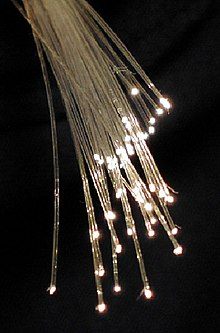
\includegraphics[scale=0.4]{./graphics/opticalfiber1}
\caption{Optical fiber}
\end{figure}

Knowledge of electromagnetic waves is required to investigate the propagation of light inside a fibre optic material. Fibre optic cable is made up of very thin hollow glass strands in which light is reflected internally. As the light propagates inside the optical fibre, the signal gets distorted and hence the knowledge of electromagnetism is needed to know how the signal gets distorted.

\section{Wireless communication}

Wireless communication is used in cell phones and most modern systems like home entertainment systems using Bluetooth speakers, laptops using a wireless method to connect to routers and so on. All these work on the principle of electromagnetic waves.
\begin{figure}[h]
\centering
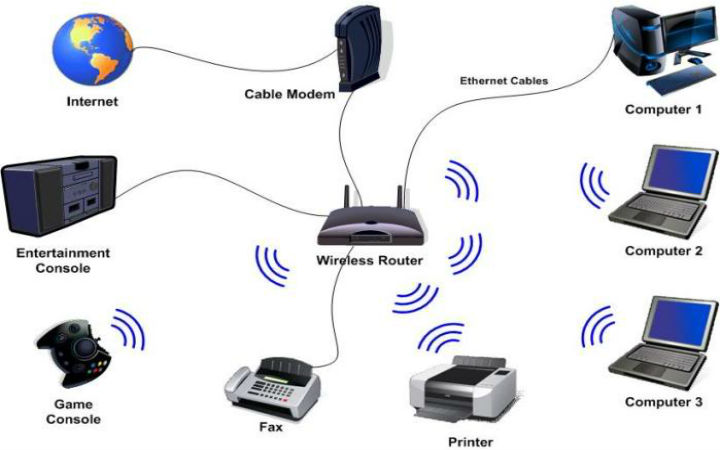
\includegraphics[scale=0.3]{./graphics/Expert-support-for-wireless-communication-projects}
\caption{Wireless connection od devices}
\end{figure}
\section{Cellular communication} 

In cellular communication, we have the base station from where the signals are transmitted, all users located inside are called a cell. Any mobile call made goes from the handset to the base station in that sector and then goes to the desired handset in the sector.
\begin{figure}[h]
\centering
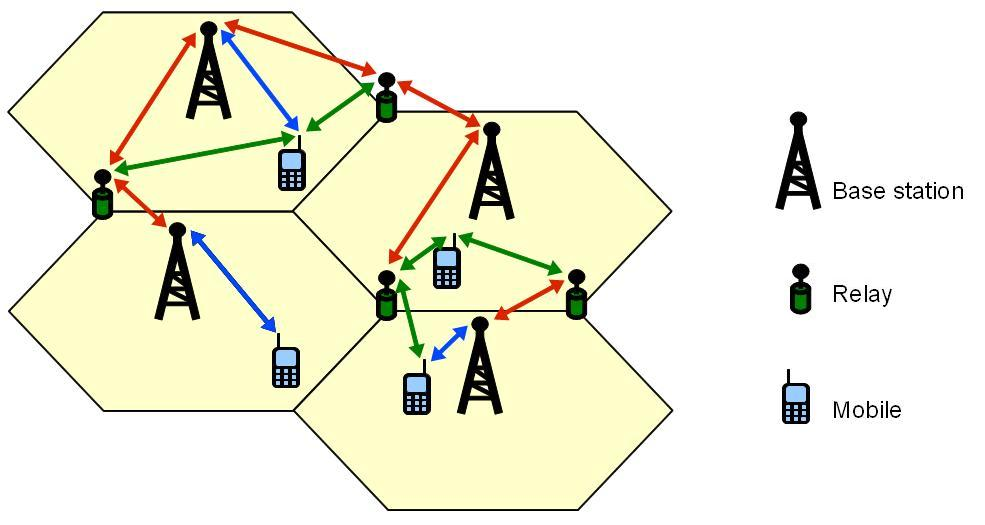
\includegraphics[scale=0.3]{./graphics/RR_sada_fig1}
\caption{Cellular communication}
\end{figure}

It is observed that a cell phone user has signals from multiple paths all coming to his cell phone\footnote{Relays are used to transmit and receive information between the base station and mobile when they are too far away to send the information to each other directly}. The mobile does not only get signals coming directly from the base station, but It also encounters signals due to reflection from associated objects. As a result of interference of these signals which can either be constructive or destructive, the final signal transmitted/received is altered. 

When there is constructive interference, a strong signal strength is observed and when the interference is destructive, a weak signal strength is observed.
The gradual weakening of a signal due to destructive interference is called \textit{fading}. To understand fading phenomenon a good knowledge of electromagnetic waves is required.\\\\

\textbf{Antennas and antenna systems for cellular communication}: To avoid fading phenomena, antennas in the mobile use sectioned propagation pattern. This implies that the cell phone gets its signal from the base station directly while minimizing signals from paths not in the direction of the base station of the antenna. A good knowledge of electromagnetic waves is required to design this system.
\begin{figure}[h]
\centering
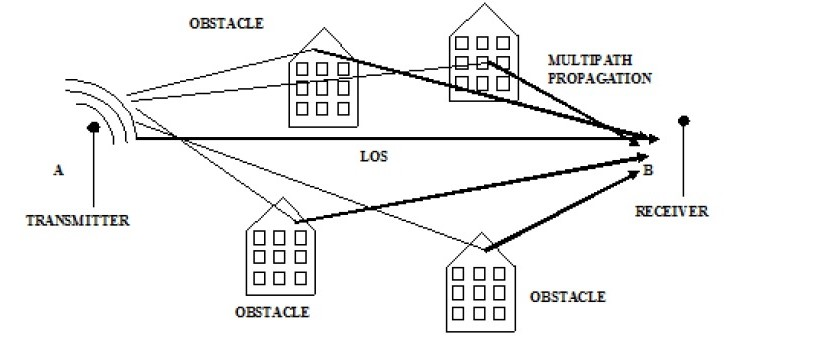
\includegraphics[scale=0.4]{./graphics/rod}
\caption{Illustration of signal inference}
\end{figure}
\section{Radar and remote sensing}
In radar altimetry, electromagnetic waves are used for finding the distance of an object from the point to the antenna. The antenna is excited with an electromagnetic pulse and the dish beams parallel waves downwards. This beam is reflected from the earth's surface back to the dish. The dish converges the received signal back to the antenna, Resulting signals are now processed in the detector, see figure 1.15.
\begin{figure}[h]
\centering
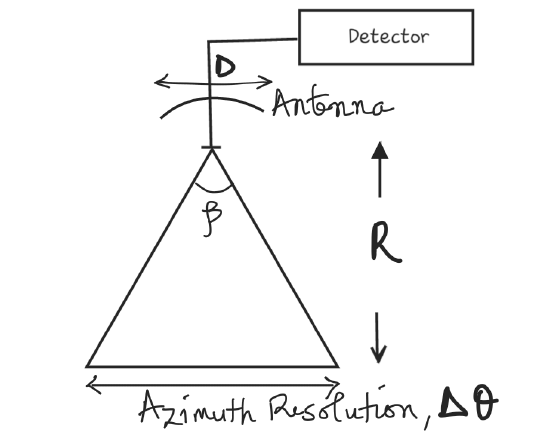
\includegraphics[scale=0.6]{./graphics/New}
\caption{Radar Altimetry}
\end{figure}

where the resolution $\Delta \theta = \frac{\lambda}{D}$\footnote{The implication of this equation lies in the size of the antenna. To get a high resolution the size of the antenna would be large}, $\lambda$ is the wavelength of the beam and $D$ is the size(length) of the antenna. 
From the time delay($\frac{C t}{2}$) of transmission to the reception of the electromagnetic pulse. The distance travelled by the beam can be estimated and also if the object is moving in the radial direction, there would be a frequency change between the signal transmitted by the antenna and the signal reflected(Doppler shift) and from this result the velocity of the object can be estimated. The radar essentially uses the electromagnetic pulse to find the distance and the velocity of an object.\\

\textbf{The monostatic radar equation}
\begin{figure}[h]
\centering
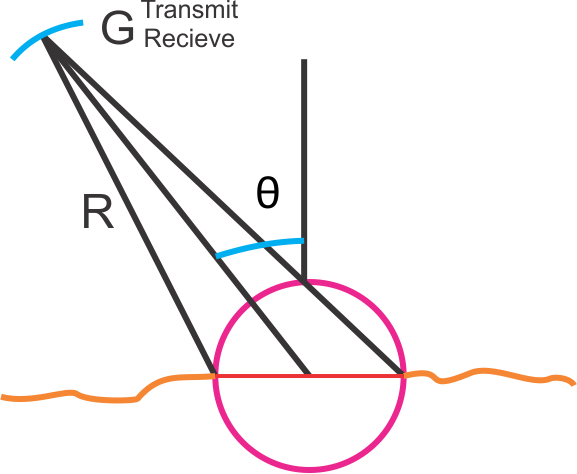
\includegraphics[scale=0.4]{./graphics/new1}
\label{fig:new1}
\caption{}
\end{figure}
\begin{center}
$p_{r}= \frac{\lambda^{2} G \delta \sigma A}{(4\pi)^{2}R^{2}}$
\end{center}

From Figure~\ref {fig:new1}, where $p_{r}$ is the received power, the signal goes from the radar to the object and is again received by the antenna in the radar. The magnitude of the received signal can be calculated and this requires a good knowledge of the ability to model the propagating environment and a good modelling of the scatterer from which the energy is going to be reflected.\\

\begin{figure}[h]
\centering
\includegraphics[scale=0.5]{./graphics/Radarlocator}
\caption{radar locator}
\label{fig:radarlocator}
\end{figure}

In Figure~\ref{fig:radarlocator}, we can see the various objects detected by the radar(represented by a green dot). The green radial line represents the transmitting beam\\

\textbf{Side looking airborne radar(SLAR):} is a radar technique used for remote sensing, it is an imaging radar\footnote{Imaging radar provides its light to illuminate an area on the ground and takes the picture at radio wavelengths} mounted on a moving object like the aircraft pointing perpendicular to the direction of flight (hence side-looking). A squinted (non-perpendicular) mode is possible also. SLAR can be fitted with a standard antenna (real aperture radar) or an antenna using synthetic aperture(this would be discussed in the next section). The platform of the radar moves in direction of the x-axis. The radar looks with the looking angle $\theta$ (or so-called off-nadir angle).\\

The microwave beam is transmitted obliquely at right angles to the direction of flight illuminating a swath.\\
Swath width refers to the strip of the Earth's surface from which data are collected by a side-looking airborne radar. It is the width of the imaged scene in the range dimension. The longitudinal extent of the swath is defined by the motion of the aircraft with respect to the surface, whereas the swath width is measured perpendicularly to the longitudinal extent of the swath. Range refers to the across-track dimension perpendicular to the flight direction, while azimuth refers to the along-track dimension parallel to the flight direction\footnote{This technique is mostly used in aircraft}.\\

\textbf{\textit{To measure the azimuth resolution}}\\
The SLAR is primarily a real aperture radar. This requires a reasonably large antenna for adequate angular resolution. The azimuth resolution, $ Ra $, is defined as
\begin{center}
$R_{a}=\frac{H \lambda}{L cos\theta}$
\end{center}
$ H $ is the height of the antenna(height of the airplane)\\
$ D $ is the geometric length of the antenna,\\
$\lambda$ is the wavelength of the transmitted pulses, and\\
$\theta$ is the incidence angle
\begin{figure}[h]
\centering
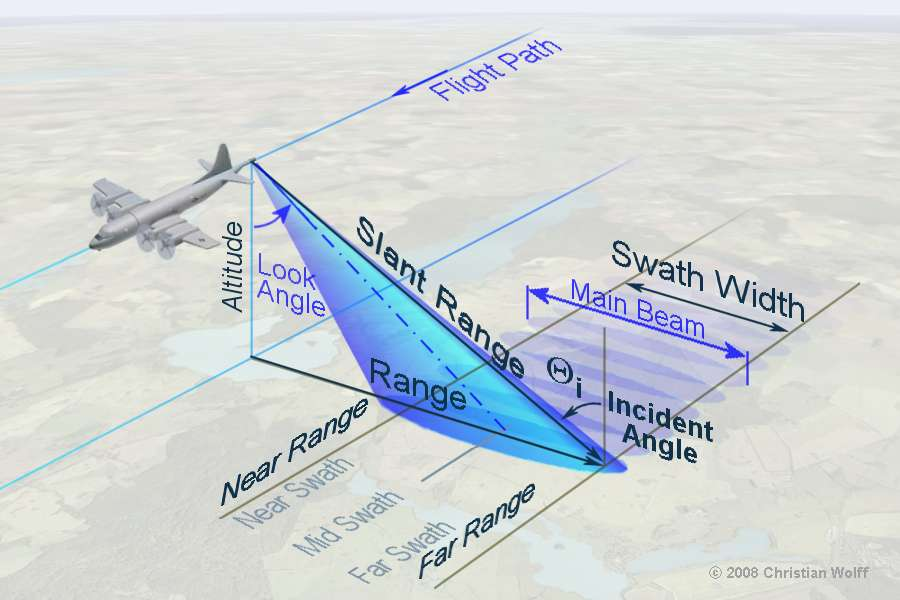
\includegraphics[scale=0.2]{./graphics/SLAR2}
\caption{Diagram expressing the SLAR}
\end{figure}

The equation shows, that increasing altitude decreases the azimuthal resolution of SLAR. A very long antenna (i.e., large D)\footnote{For this book, $D$ is the size of the antenna. hence the statement "large D", since the length ($L$) of an object is a function of the size ($D$)} would be required to achieve a good resolution from the aircraft. Synthetic Aperture Radar (SAR) is used to acquire higher resolution.\\

\textit{\textbf{To measure the cross-track resolution }}\\
At all ranges, the radar antenna measures the radial line of sight distance between the radar and each target on the surface. This is the slant range distance. The ground range distance is the true horizontal distance along the ground corresponding to each point measured in the slant range. The cross-track resolution, $R_{r}$, is defined as:  
\begin{center}
$R_{r}=\frac{c_{0} t_{p}}{2 sin\theta}$
\end{center}
$c_{0}$ is the speed of light\\
$t_{p}$ is the pulse duration of the transmitter and\\
$\theta$= incidence angle

\begin{figure}[h]
\centering
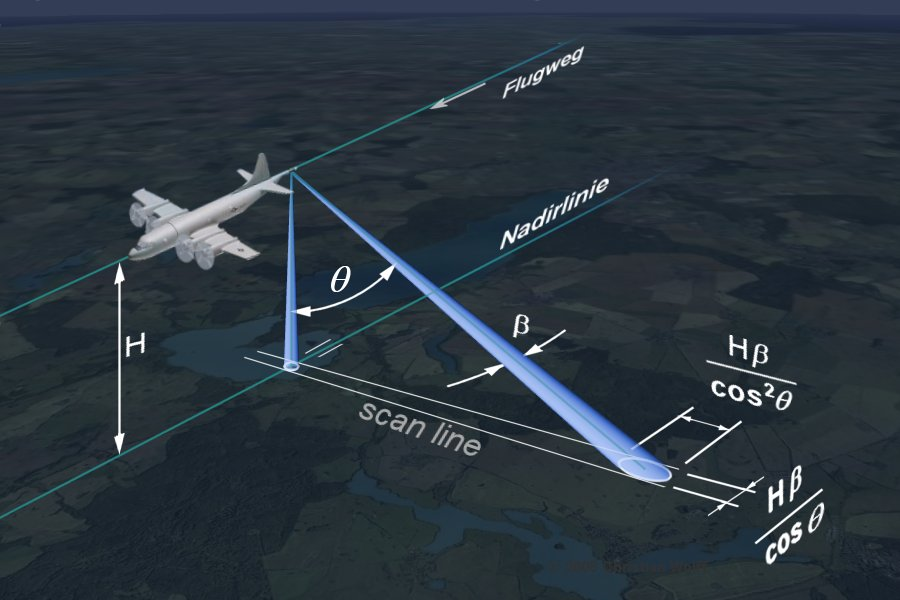
\includegraphics[scale=0.2]{./graphics/SLAR-resolution}
\caption{Diagram expressing the SLAR}
\end{figure}
\textbf{Synthetic aperture radar(SAR):} To improve the resolution in remote sensing, a technique called the synthetic aperture dish is used. For an antenna like a parabolic dish, the angular resolution is given as the wavelength divided by the size\footnote{For a parabolic dish antenna the diameter 'd' is used instead of length 'L'.See footnote 11} for the antenna, $\Delta \theta = \frac{\lambda}{D}$. To get a fine resolution for the image in remote sensing, a very large aperture D is required. A large D cannot be easily created especially in moving vehicles and aircraft.\\

A technique where the antenna is small but the vehicle moves and as the vehicle moves, the reflection information is stored after all the refection information is collected from different locations, then data processing can be done to get an angular resolution which will correspond to the total distance traveled by the vehicle. This technique is known as the \textit{synthetic aperture radar}.
\begin{figure}[h]
\centering
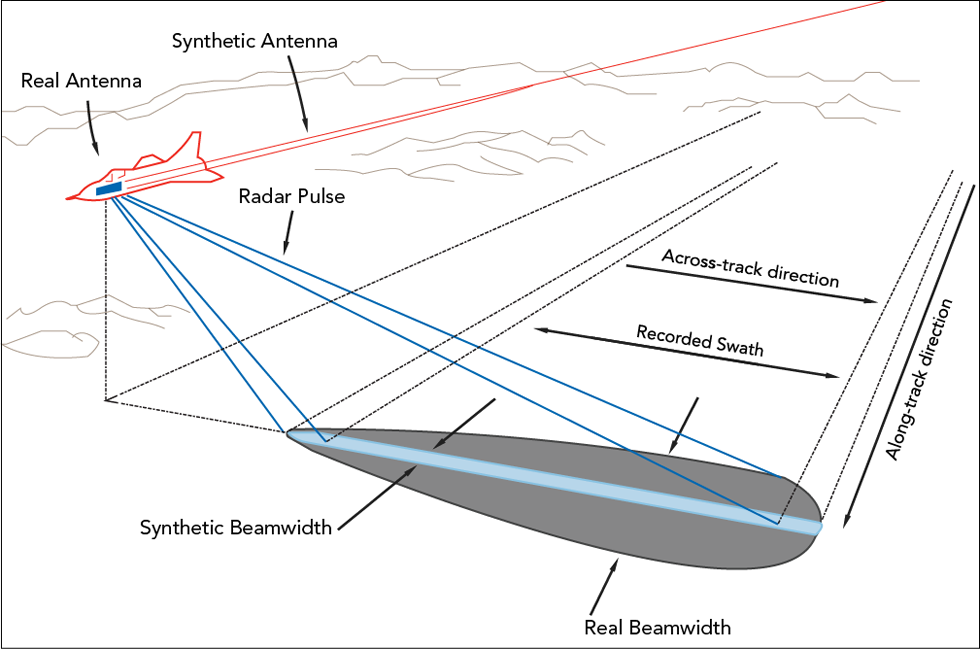
\includegraphics[scale=0.3]{./graphics/sar2}
\caption{Diagram expressing the SAR}
\end{figure}

\textbf{SAR features}
\begin{enumerate}
\itemsep0em
\item very high linear resolution independent of the range
\item requires a source with higher coherence
\item image is on the range-doppler coordinate grid
\item requires a large data processing
\item geometric and ratio metric distortions
\item speckle noise
\end{enumerate}

\section{Radio astronomy} 

A typical radio telescope is shown below with a passive receiver. In this case, no signal is transmitted but the signal is received.\\
\begin{figure}[h]
\centering
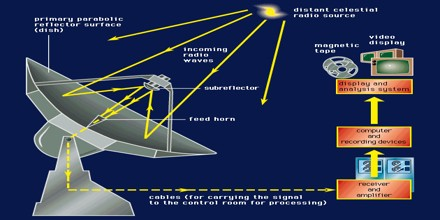
\includegraphics[scale=0.5]{./graphics/Radio-Telescope-0}
\caption{Radio telescope}
\end{figure}

The frequency of the signals is converted, detected and processed. With a radio telescope, we would like to get an image of the sky with as large a resolution as possible.

$\frac{\lambda}{D}$ comes into the picture and to get a very fine resolution of the image of the sky, a very large telescope would be needed.

Producing a very large telescope is difficult so we use the aperture synthetic technique as it was used on radars. In this method we use a set-up of antennas, for example, if the dish in each array is of the order of $ D = 25m $ and the total spread of the antennas of the order 21km. Therefore, we get an effective aperture through each antenna that has an aperture of only 25m.

\section{EMI/EMC}

\textbf{EMI} is electromagnetic interference.
Firstly, let us investigate how a high-frequency device would create interfering signals and then what ways in which the interference can be reduced.

For example, you may get interference on our radios, whenever somebody starts a car or a motorcycle in the vicinity, because starting a car or motorcycle involves sparking and because of that spark, you get electromagnetic interference which is picked up by the radio antenna and you get disturbance on your radios. It is essential to investigate the technique by which the interferer can be reduced or the mechanism by which the devices can be isolated. This technique is called \textit{\textbf{shielding}}.\\

\textbf{EMC} is electromagnetic compatibility. Today, whenever we design electromagnetic gadgets or electrical devices it is mandatory to make them electromagnetically compliant so it does not create additional electromagnetic interference which will affect the other systems.

The figure below describes the whole concept of EMC both causes(natural or man-made) and solution(shielding and other techniques).
\begin{figure}[h]
\centering
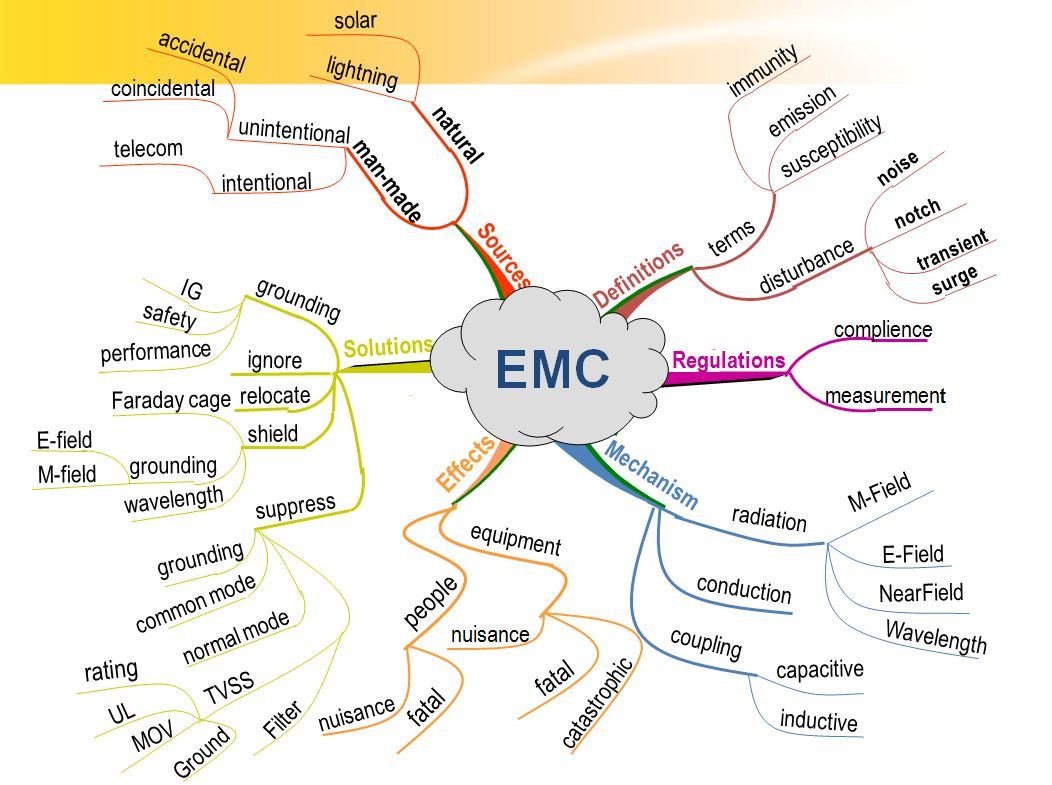
\includegraphics[scale=0.35]{./graphics/634771461726914062}
\caption{Electromagnetic Compatibility}
\end{figure}
